\section{Software design and implementation}\label{sec:design}

In this section we provide an overview of the current design of the AMIDST toolbox as well as the status of the
toolbox implementation. The first subsection gives a general overview of the core parts of the framework,
which provide the foundation for the more learning specific aspects described in the second subsection.    

\subsection{The core module}
\label{sec:core-module}

An overview of the core components of the AMIDST toolbox is illustrated in Figure
\ref{Figure:ToolboxBasicStructure}. The color coding in the figure summarizes the implementation status: blue boxes represent
software components that have been implemented in the AMIDST toolbox and green boxes represent components
that are part of the software design specification but which has not yet been implemented.      

The structures included in the figure
mainly relates to the basic components that play a key role in ensuring the
forthcoming implementation of the different AMIDST learning and inference algorithms. For starters, instantiation of a particular probabilistic graphical model (\comp{PGM} component) will be required. Currently it is possible to create either a static Bayesian network (\comp{BN} component) or a two time-slice dynamic Bayesian network (\comp{2T-DBN} component).

\begin{figure}[htbp]
\begin{center}
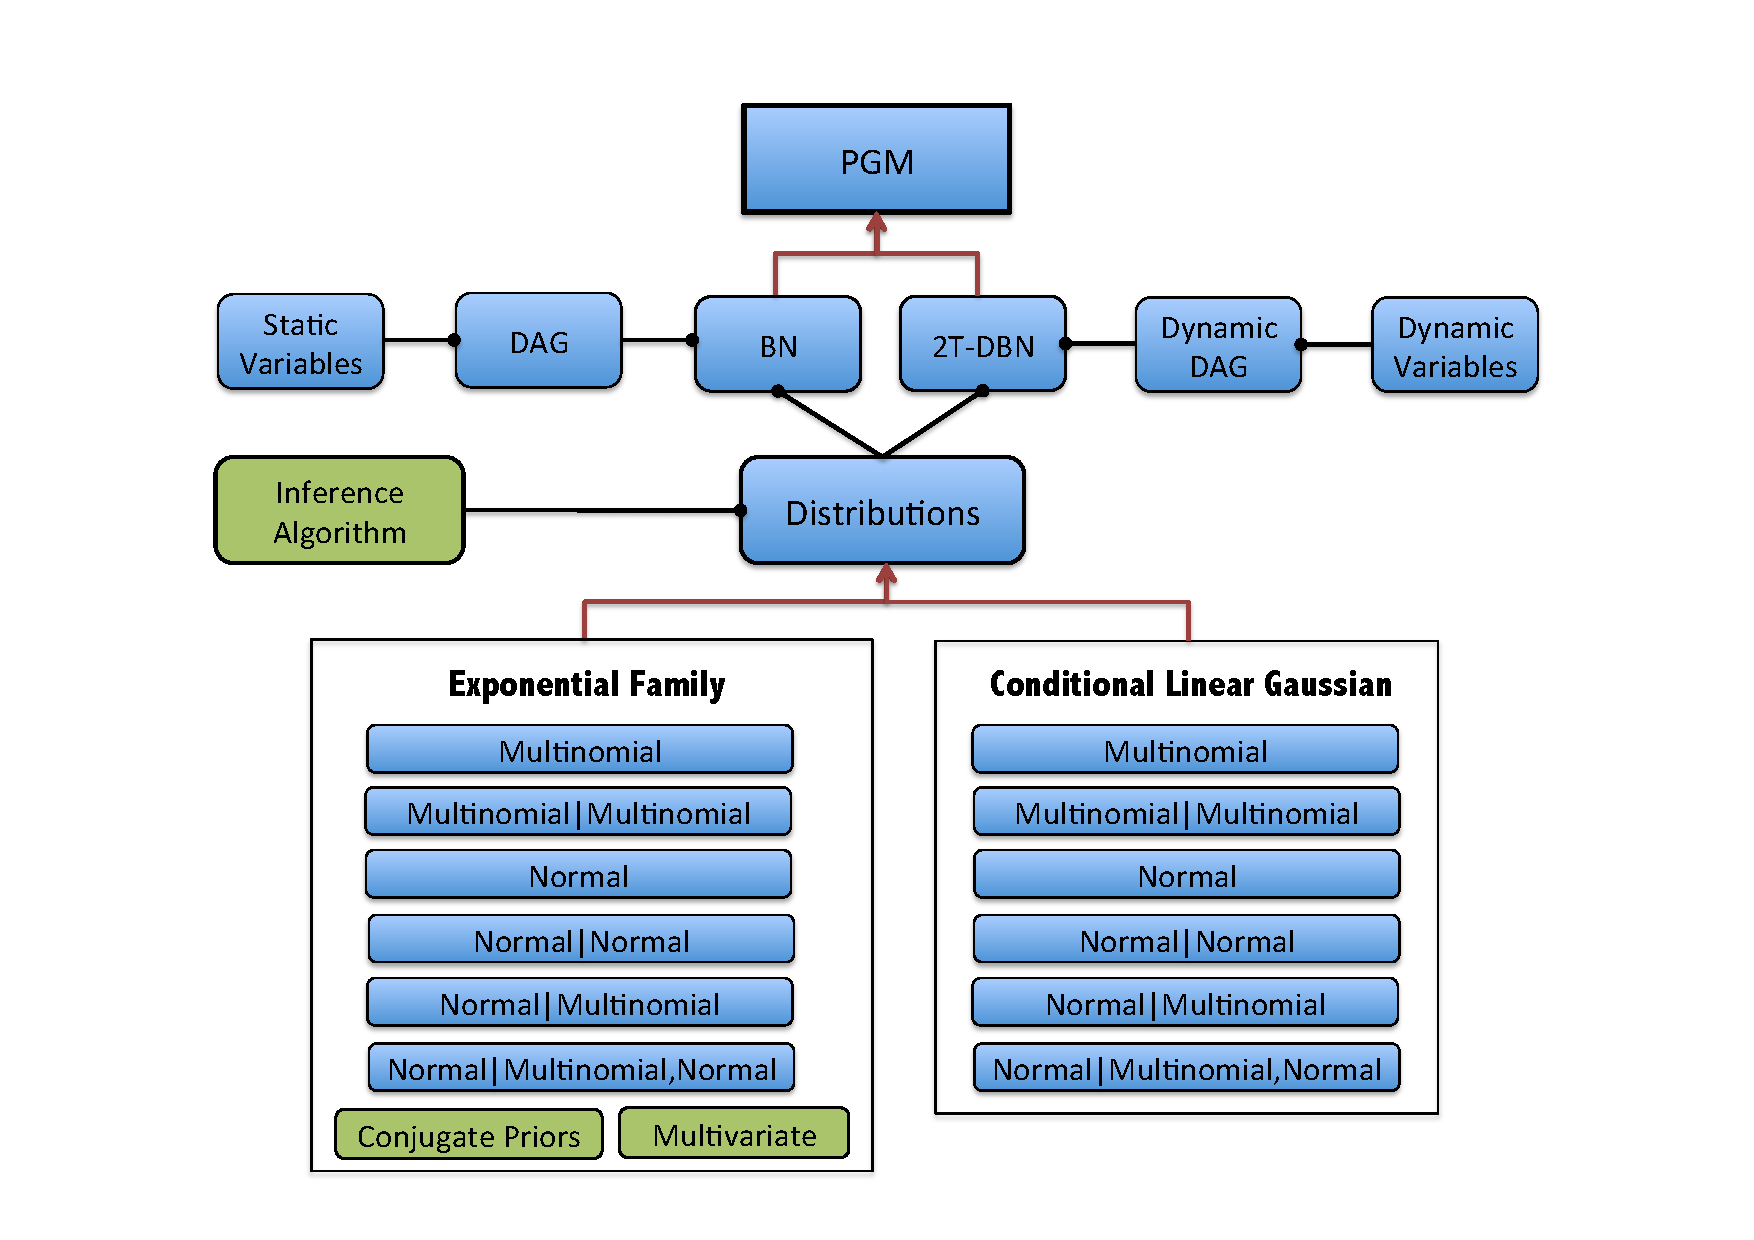
\includegraphics[width=\linewidth]{./figures/ToolboxBasicStructures}
\caption{\label{Figure:ToolboxBasicStructure} Illustration of the design of the software components related to
  core structures. Nomenclature: The boxes in the
      figure represent software components (sets, possibly singletons, of classes), a rounded-arc going from $X$
      to $Y$ indicates that $Y$ 'uses/references' $X$, and an arc with an arrow from $X$ to $Y$ implies
      inheritance.}
\end{center}
\end{figure}

As previously described in Section 2, a BN consists of two components:

\begin{itemize}
  \item A directed acyclic graph (\comp{DAG} component) defined over a list of \comp{Static Variables}. Each static variable is characterized by its name, ID, the state space type, the distribution type (i.e., multinomial or normal), as well as if it is observed or not.

  \item Conditional probability distributions of each variable given its parents (defined by the \comp{Distributions} component).
\end{itemize}

Similarly to a BN, a 2T-DBN (see Deliverable D2.1, Section 3.4 \cite{AMIDST-D21}) is defined using two main components:


\begin{itemize}
\item A dynamic acyclic graph (\comp{Dynamic DAG} component) defined over a list of dynamic variables. The
  component specifies the graph structure of a \comp{2T-DBN}, i.e. the parent set for each variable at both time $0$ and at time $t>0$. Each dynamic variable is characterized by its name, ID, the state space type, the distribution type (i.e., multinomial or normal), and if it is observed or not. In order to represent the variables in a previous time step (needed when defining the dynamic DAG), we use the concept of \textit{temporal clone} variables, which are copies of the real main variables but refer to the previous time step. For instance, $X_{t-1}$ is codified as the \textit{temporal clone} of variable $X_t$. Hence, in our data structures, the time index $t$ is not explicitly represented for a dynamic variable, but implicitly considered with the use of \textit{temporal clones}.

\item Conditional probability distributions of each variable given its parents (encoded in the \comp{Distributions} component).

\end{itemize}

Note here that, in spite of the distinction between \comp{BN} and \comp{2T-BN}, the distributions associated
with the variables in both model classes can be defined in the same way. In particular, the \comp{Distributions} component
includes the set of conditional probability distributions considered in the AMIDST toolbox. More precisely,
both variables with multinomial and normal distributions are modeled, and the distribution of each variable,
in either a BN or a 2T-DBN, is initialized and specified according to its distribution type and the
distribution types of its potential parents. This consequently gives rise to the following different
implemented probability distributions: 

% Note here that, in spite of this distinction between \comp{BN} and \comp{2T-BN}, the Distributions over both models could be defined in the same way, and thereby the parameter learning and inference algorithms could be also applied equally for both models. In particular, the \comp{Distributions} component includes the set of conditional probability distributions considered in the AMIDST toolbox (the so-called \comp{Conditional Linear Gaussian} distributions, as detailed in Deliverable 2.1). More precisely, both variables with multinomial and normal distributions are modeled, and the distribution of each variable, in either a BN or 2T-DBN, is initialized and specified according to its distribution type and the distribution types of its potential parents. This consequently gives rise to the following different implemented probability distributions:

\begin{itemize}
  \item \comp{Multinomial}: a multinomial variable with no parents.
  \item \comp{Multinomial$|$Multinomial}: a multinomial variable with multinomial parents.
  \item \comp{Normal}: a normal variable with no parents.
  \item \comp{Normal$|$Normal}: a normal variable with normal parents.
  \item \comp{Normal$|$Multinomial}: a normal variable with multinomial parents.
  \item \comp{Normal$|$Multinomial,Normal}: a normal variable with a mixture of multinomial and normal parents.
\end{itemize}

The case of a multinomial variable having normal parents is not considered yet in this initial prototype. It
is planned to be included in future versions, although strongly restricted in inference and learning
algorithms due to the methodological and computational issues previously commented in Deliverable D2.1 \cite{AMIDST-D21}. 

We also provide an implementation of all the above distributions in the so-called \comp{Exponential Family}
form, which ensures an alternative representation of the standard distributions based on vectors of natural
and moment parameters. This representation of the distributions support the type of parameter learning schemes
pursued in AMIDST (see below).


% In this case, the learning process can be efficiently carried out through Bayesian
% inference with the exponential family representation. The definition of a set of corresponding conjugate
% priors gives support to this kind of learning. It is important to notice also that the AMIDST framework
% will be flexible enough to give support to joint relationships between variables in learning (and inference)
% by defining clusters of variables or multivariate exponential family distributions.  